\newpage
\section*{Zielsetzung}
\section{Theorie}
\subsection{Aufbau}
Das Geiger-Müller-Zährohr besteht aus einem, mit einem Gasgemisch gefülltem,
Hohlzylinder. Der Mantel des Zylinders bildet dabei die Kathode (bei einem Radius $r_k$).
Im Zentrum des Volumen bildet ein Draht die Anode mit dem Radius $r_a$. Eine angelegte
Spannung $U$ erzeut somit ein radialsymmetrisches elektrisches Feld.\\
Die eine Seite des Zylinders ist verschlossen, während die andere Seite über ein 
Maylarfenster verfügt. Durch die geringe Massendichte, kann somit ionisiernde Strahlung durch
dieses dünne Material einfallen.

\begin{figure}
    \centering
    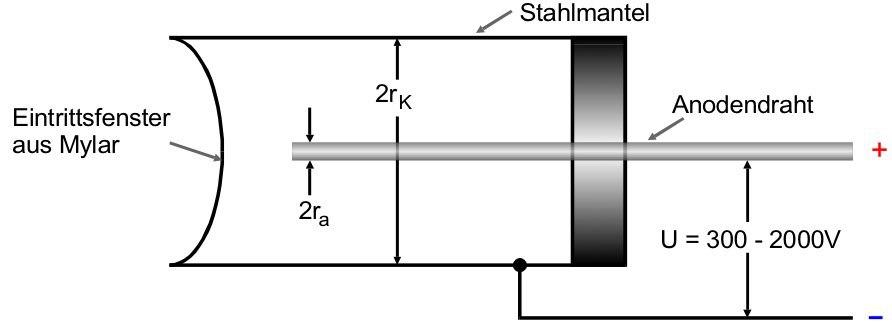
\includegraphics[width=0.7\textwidth]{input/querschnitt.jpg}
    \caption{Dargstellt ist der Querschnitt eines Geiger-Müller-Zählrohres mit
    dem Anodendraht, dem Kathodenzylinder und dem Mylarfenster.\cite[220]{anleitung}}
\end{figure}
\subsection{Funktionsweise und Ansprechvermögen}
Die Wahrscheinlichkeit, dass ein Teilchen im Zählrohr nachgewiesen wird,
versteht man als Ansprechvermögen. Während bei $\alpha$- und $\beta$-Teilchen, aufgrund
ihres hohen Ionisationsvermögens, der Nachweis bei nahzu 100\% liegt, ist das 
Ansprechvermögen für Photonen mit Materie kleiner (ca. 1\%,lediglich hohe $\gamma$-
Intensitäten können vermessen werden).\\
Tritt ein Teilchen, welches die Gasatome ionisieren kann, in die Kammer ein, so
ionisiert es Atome des entahteten Gasgemisches (unteranderem Argon). Dies tut 
das Teilchen so oft, bis dieses so wenig Energie besitzt, um weitere Ionisationen durchzuführen. 
Die frei gewordenen Elektronen beschleunigen aufgrund des angelegten Feldes auf die 
Anode zu. Treffen mehrere Elektron dort auf, kann dies als Impuls regristriert werden.
Für eine Ionisationen eines Argon Atoms sind im Durchschnitt $26\si{ev}$ nötig.
Über die Anzahl der regristrierten Impulse, kann somit auf die Energie des eingefallenden Teilchens
zurückgeschlossen werden. Es gilt, die Anzahl der Ionisationen sind proportional zu
der Energie des einfallenden Teilchens, wenn gleich die gemessenen Impulse 
auch stark von der anglegten Spannung $U$ abhängen.

\subsection{Spannungsabhängigkeit}
Wie oben erwähnt, sind die Anzahlen der gemessenen Impulse stark von 
der angelegten Spannung abhängig. Die verschieden hohen Betriebsspannungen $U$ 
führen zu verschiedenen Effekten, die in 5 Bereichen aufgeteilt werden können.

\begin{figure}
    \centering
    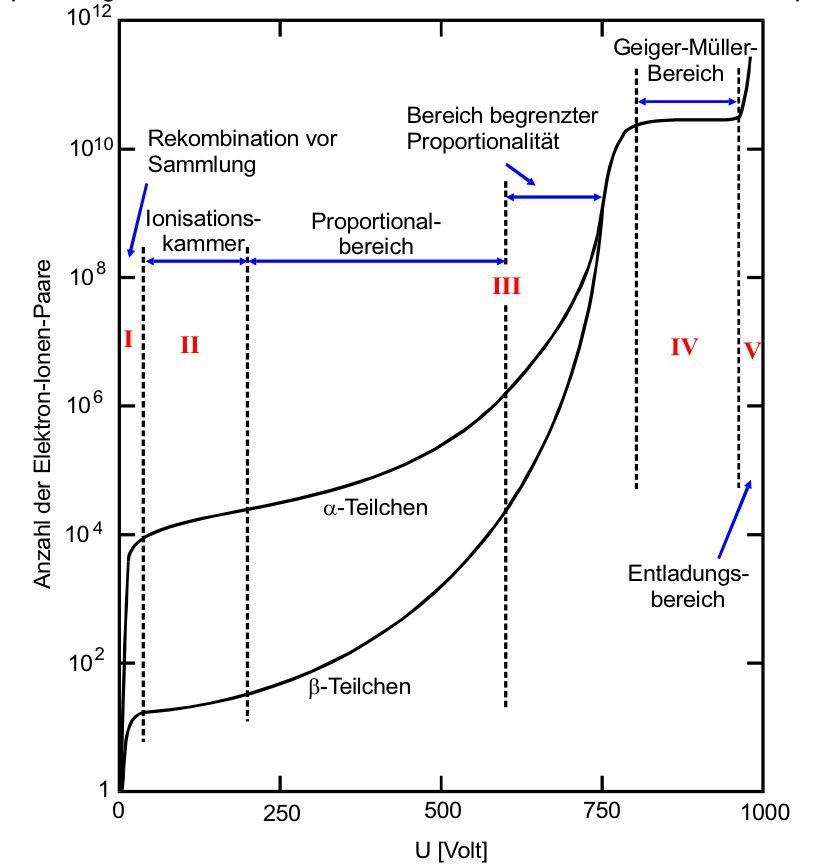
\includegraphics[width=0.7\textwidth]{input/bereiche.jpg}
    \caption{Dargestellt ist die Anzahl der erzeugten Elektron-Ionenpaare als Funktion der Spannung $U$
    für ein Proportionalzählrohr\cite[221]{anleitung}}
    \label{fig:bereiche}
\end{figure}
\subsubsection*{Bereich 1}
Ist die Zählrohrspannung klein (vgl. Bereich 1 in Abb. \ref{fig:bereiche})
so erreichen nur wenige der frei gewordenen Elektronen den Anodendraht, da 
sie aufgrund von Rekombinationen wieder verlohren gehen.
\subsubsection*{Bereich 2 - Ionisationskammer}
Mit höherer Zählrohrspannung nimmt die Rekombinationswahrscheinlichkeit ab und
es kommen nahzu alle Elektronen zum Anodendraht. Hierbei ist dann der entstandene
Ionisationsstrom proportional zur Energie und zur Intensität der einfallenden Teilchen.
Da die Ionisationsströme allerdings klein sind, benötigt es große Strahlungsintensitäten.
\subsubsection*{Bereich 3 - Proportionalzählrohr}
Die Feldstärke ist hierbei groß genug, sodass die freien Elektronen neben den Zusammenstößen
mit den Argon-Atomen auch genügend Energie besitzen, um weiter Atome zu ionisieren. Diese 
Stoßionisation löst wiederrum Elektronen, die den gleichen Prozess durchlaufen, sodass es zu einer Townsend-Lawine
kommt. Pro einfallendem Teilchen kommt es somit zu einer Ansammlung an Ladung $Q$ an der Anode,
,sodass dies als Impuls wahrgenommen werden kann. Dabei ist $Q$ proportional zur
Energie des einfallenden Teilchens.
\subsubsection*{Bereich 4 - Geiger-Müller-Zähler}
Oberhalb des Proportinalbereichs ist die Ladung $Q$ unabhängig von der
Primärionsiation. Die Entladung findet hierbei nicht auf lokalisierten Elektronelawinen statt,
sonder aufgrund von UV-Photonen , die bei der Anregung von Argon mit Elektronen entstehen,
ausgedehnt längs des gesamten Zählrohres. Die UV-Photonen sind somit aufgrund ihrer Ladungsneutralität
Ursprung der Elektronenlawinen im gesamten Zählrohr.\\
Die am Ende gesammelte Ladung ist nun vom Volumen des Zählrohres und dessen Spannung abhängig und kann
nur noch zur Intensitätsmessung der eingetroffenen Strahlung verwendet werden und nicht zur Messung derer
Energie.
\subsubsection*{Bereich 5 - Entladungsbereich}
Hier ist nun die Betriebssannung $U$ so groß, dass durch ein geladenes Teilchen eine
selbstlaufende Ionisation ausgeführt wird, die zur Dauerentladung führen kann.
Der entstehende hohe Ionisationsstrom kann dabei so groß sein, dass er das
Messgerät zerstört.
\subsection{Totzeit}
Aufgrund der großen Masse der Ionen fließen diese nicht direkt zur Kathode ab, es 
entsteht eine positive Raumladung. Das führt zu einem vorübergehenden Stop der Stoßionisation.
Somit wird eintreffene Strahlung nicht detektiert.\\
Erst nachdem die Ionen zum Zylindermatel gewandert sind, steigt die Feldstärke 
an, was eine Lawinienbildung wieder möglich macht. Diese Zeit nennt man Totzeit $T$.
\\Die Totzeit verfälscht somit die Intensität $N$. Für die tatsächliche einfallende Inetensität $N_W$
gilt
\begin{equation}
    N_W=\frac{N_r}{1-TN_r},
\end{equation}
wobei $N_r$ die gemessene (verfälschte) Intensität ist.
Für die gemeinsame Impulsrate $N_{1+2}$ zweier Quellen $N_1$ und $N_2$ folgt für
die Totzeit $T$
\begin{equation}
    T \approx \frac{N_1+N_2-N_{1+2}}{2\cdot N_1N_2},
    \label{eqn:2Quellen}
\end{equation}
mit der Annahme $T^2N^2>>1$.
\subsection{Erhohlungszeit}
Die Ionen müssen vollständig neutralisiert sein, damit die Ladungsimpulse $Q$ wieder
ihre volle Höhe erreichen, wenn Strahlung erneut eintrifft.
\begin{figure}[H]
    \centering
    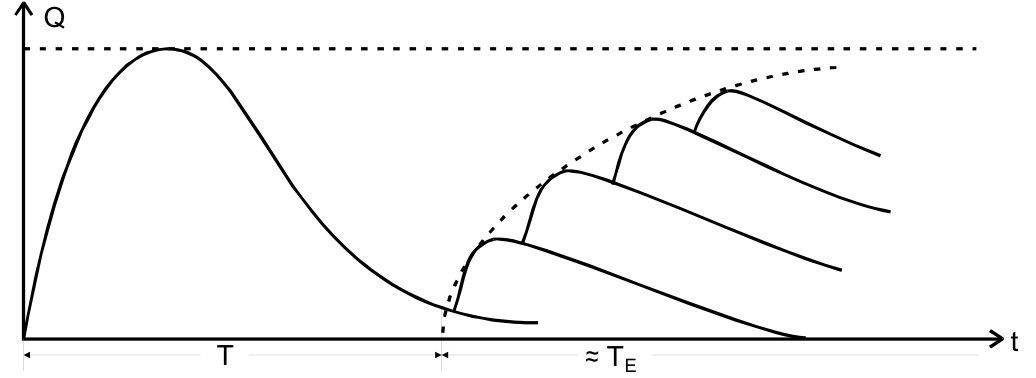
\includegraphics[width=0.7\textwidth]{input/erhohlungszeit.jpg}
    \caption{Dargestellt ist der Unterschied zwischen Totzeit $T$ und der Erhohlunszeit $T_E$.
    Die Erhohlungszeit lässt sich in der Praxis nur ungenau bestimmen.\cite[223]{anleitung}}
\end{figure}
Die Zeit zum Erreichen der ursprünglichen Ladungsimpuls $Q$ Höhe nennt man Erholungszeit $T_E$.
Diese schließt sich der Totzeit an.
\subsection{Nachentladung}
Treffen Ionen auf den Kathodenmatel, so können sie Elektronen aus der 
Metalloberfläche lösen. Diese Sekundärelektronen können somit, nach Eintreffen der Strahlung,
zu weiteren Ausgangsimpulsen zu einem späteren Zeitpunkt führen. Somit folgt auf das
Eintreffen eines einzelnen Teilchens zusätzliche Impulse.\\
Um diese Störsignale zu vermeiden, füge man Alkohldämpfe zum Argongas hinzu.
Dies hat den Effekt, dass die Alkohlmoleküle bei einem Zusammenstoß mit den Argonatomen ionisiert werden
und dann zur Kathode laufen. Aufgrund ihrer Struktur, führen die freiwerdenen Elektronen nicht zur
Aussendendung eines weiteren Elektrons, sondern zur Schwingungsanregung.
Somit werden keine neuen Elektronen aus der Kathode freigesetzt und die Nachentladung erlischt. 

\subsection{Charakteristik}
Die Charakteristik erhält man durch Auftragen der regristrierten Teilchenzahl $N$
gegen die angelegte Betriebsspannung $U$ bei konstanter Strahlunsintensität der Quelle.
Der mittlere lineare Teil der Kurve (vgl. Abb \ref{fig:charakter}) wird Plateau genannt.
Je näher dessen Steigung bei null ist und je länger dessen Verlauf, desto besser (idealer) arbeitet 
das Zahlrohr.
\begin{figure}
    \centering
    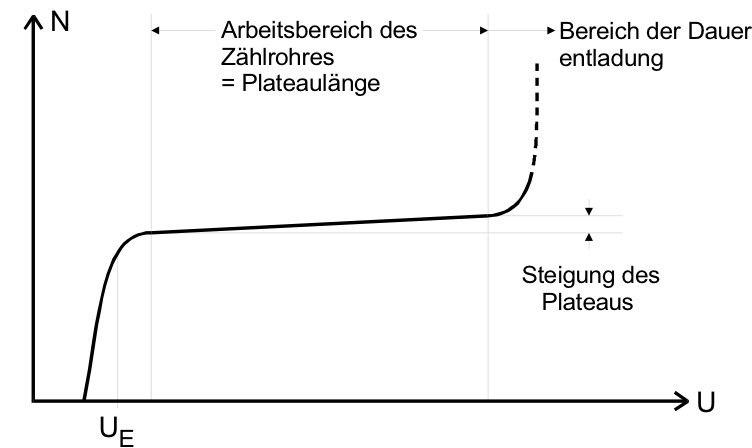
\includegraphics[width=0.7\textwidth]{input/charakteristik.jpg}
    \caption{Gezeigt ist die Zählrohrcharakteristik.\\
    Bei der Spannung $U_E$ setzt der Auslösebereich ein, gefolgt von dem
    Plateau. Am Ende nimmt die gemessene Teilchenzahl $N$ wieder zu.
    Dies resultiert aus einer gezündeten Dauerentladung ionisierender Teilchen,
    die zu einer selbständigen Gasentladung führt.\cite[224]{anleitung}}
\end{figure}
Über den Anodenstrom $I$ lassen sich die freigesetzten Ladungen pro einfallendem Zeilchen Z
ermitteln.
\begin{equation}
    Z=\frac{I}{eN},
    \label{eqn:strom}
\end{equation}
wobei $N$ die gemessene Impulsrate und $e$ die Elementarladung ist.
